\section{Erro nas Comunicações}

\begin{frame}[allowframebreaks]
  \frametitle{Erro nas Comunicações}

  \begin{figure}[h!]
  \centering
  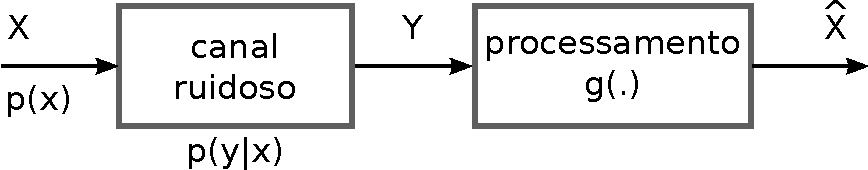
\includegraphics[width=0.7\textwidth]{images/canal-ruidoso.pdf}
  %\caption{.}
  \label{fig:canal-ruidoso}
  \end{figure}

  \begin{itemize}
        \item $\hat{X}$ é uma estimativa de $X$.
        \item a estimativa é errada quando $X \neq \hat{X}$
        \item probabilidade de erro: $P_e \triangleq p(X \neq \hat{X})$
        \item podemos relacionar a entropia condicional $H(X|Y)$ com a probabilidade de erro $P_e$?
        \item sabemos (exercício anterior) que a entropia condicional $H(X|Y)$ é nula se e somente
        se $X$ for uma função de $Y$
        \item esperamos ser capazes de estimar $X$ com baixa probabilidade de erro apenas quando
        a entropia condicional $H(X|Y)$ for pequena
  \end{itemize}
\end{frame}

\subsection{Desigualdade de Fano}

\begin{frame}%[allowframebreaks]
  \frametitle{Desigualdade de Fano}
  \begin{theorem}[Desigualdade de Fano]
  Para qualquer estimador $\hat{X}$ tal que $X \rightarrow Y \rightarrow \hat{X}$, com
  $P_e = Pr(X \neq \hat{X})$, temos
  \begin{equation}
        H(P_e) + P_e \log \left( \vert \mathcal{X} \vert - 1 \right) \geq H(X|\hat{X}) \geq H(X|Y)
  \end{equation}
  Esta desigualdade pode ser simplificada (menos rígida) na forma
  \begin{equation}
  P_e \geq \frac{H(X|Y) - 1}{\log \left( \vert \mathcal{X} \vert - 1 \right)}
  \label{eq:desfanorelax}
  \end{equation}
  onde utilizamos $H(P_e) \leq 1$.
  \end{theorem}
  Note que $P_e = 0 \Rightarrow H(X|Y)=0$ pois $H(P_e)=0$ e $H(X|Y) \geq 0$.
\end{frame}
\note{
Esta desigualdade será utilizada para provar o reverso no teorema de codificação
de Shannon, i.e., que qualquer código com probabilidade de erro $\rightarrow 0$,
à medida que o comprimento do bloco cresce, devemos ter uma taxa $R < C$
(a capacidade do canal, a ser definida).

Para o caso de um alfabeto binário ($\vert \mathcal{X} \vert = 2$),
a desigualdade de Fano na forma da Equação \ref{eq:desfanorelax}
não poderá ser aplicada. Devemos então utilizar a forma mais relaxada:
  \begin{equation}
  P_e \geq \frac{H(X|Y) - 1}{\log \left( \vert \mathcal{X} \vert - 1 \right)} 
        > \frac{H(X|Y) - 1}{\log \vert \mathcal{X} \vert }
  \end{equation}

}

\begin{frame}[allowframebreaks]
  \frametitle{Desigualdade de Fano}
  \begin{proof}
        Definir uma função de erro:
        \begin{equation}
        E = \begin{cases} 1 &, \text{ se } \hat{X} \neq X \text{(erro)} \\
                0       &, \text{ se } \hat{X} = X \text{(sem erro)} 
        \end{cases}
        \end{equation}

        \proofbreak

        Utilizando a regra da cadeia temos:
        \vspace{-0.3cm}
        \begin{eqnarray}
        H(E,X|\hat{X}) &=& H(X|\hat{X}) + \underbrace{H(E|X,\hat{X})}_{=0} \nonumber \\
                        &\text{ou}& \nonumber \\
                        &=& \underbrace{H(E|\hat{X})}_{\leq H(E) = H(P_e)} + \underbrace{H(X|E,\hat{X})}_{\leq P_e \log (\vert \mathcal{X} \vert - 1)}
        \end{eqnarray}
        \vspace{-0.3cm}
        \begin{itemize}
        \item O erro é uma função determinística de $X$ e $\hat{X}$, então, sabendo $X$ e $\hat{X}$,
                determinamos $E$. Desta forma: $H(E|X,\hat{X})=0$.
        \item Condicionar só pode reduzir a entropia: $H(E|\hat{X}) \leq H(E) = H(P_e)$.
        \item Veremos abaixo que $H(X|E,\hat{X}) \leq P_e \log (\vert \mathcal{X} \vert - 1)$.
        \end{itemize}

        \proofbreak

        \vspace{-0.3cm}
        \begin{eqnarray}
        H(X|\hat{X},E) &=& p(E=0) \underbrace{H(X|\hat{X},E=0)}_{=0} + p(E=1)H(X|\hat{X},E=1) \nonumber \\
                        &=& (1-P_e) 0 + P_e H(X|\hat{X},E=1) \leq P_e \log (\vert \mathcal{X} \vert - 1) \nonumber
        \end{eqnarray}
        \begin{itemize}
        \item Se não há erro e conhecemos $\hat{X}$, então determinamos $X$. Não existe entropia 
                residual em $X$ quando é dado $\hat{X}$ e $E=0$. Logo $H(X|\hat{X},E=0)=0$.
        \item Se conhecemos $\hat{X}$ e existe um erro ($E=1$), então sabemos que
                $X$ é diferente de $\hat{X}$, logo isto nos deixa com $(\vert \mathcal{X} \vert - 1)$
                alternativas.
        \end{itemize}

        \proofbreak

        Temos então
        \begin{eqnarray}\label{eq-hhpelog}
        H(X|\hat{X}) &=& H(E|\hat{X}) + H(X|E,\hat{X}) \nonumber \\
                &\leq& H(P_e) + P_e \log (\vert \mathcal{X} \vert - 1)
        \end{eqnarray}

        Como $X \rightarrow Y \rightarrow \hat{X}$ é uma cadeia de Markov, podemos utilizar a
        desigualdade de processamento de dados.
        \begin{eqnarray}\label{hxxhxy}
        I(X;Y) &\geq& I(X;\hat{X}) \nonumber \\
        H(X) - H(X|Y) &\geq& H(X) - H(X|\hat{X}) \nonumber \\
        H(X|\hat{X}) &\geq& H(X|Y)
        \end{eqnarray}

        \proofbreak

        Então, utilizando as Equações \ref{eq-hhpelog} e \ref{hxxhxy}, obtemos
        \begin{equation}
        H(P_e) + P_e \log (\vert \mathcal{X} \vert - 1) \geq H(X|\hat{X}) \geq H(X|Y)
        \end{equation}
        
  \end{proof}
\end{frame}

\begin{frame}%[allowframebreaks]
  \frametitle{Desigualdade de Fano - Sumário}
  Considere a seguinte situação: enviamos $X$ através de um canal ruidoso,
  recebemos $Y$ e realizamos algum pós-processamento.
  \begin{figure}[h!]
  \centering
  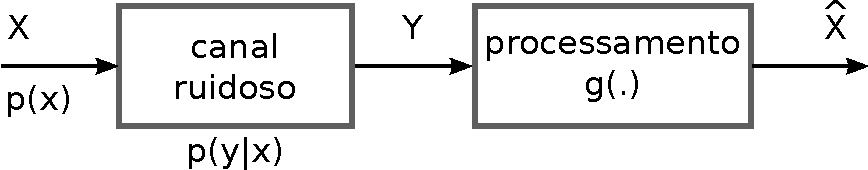
\includegraphics[width=0.8\textwidth]{images/canal-ruidoso.pdf}
  %\caption{.}
  \label{fig:canal-ruidoso}
  \end{figure}
  $\hat{X}$ é uma estimativa de $X$.
  \begin{itemize}
  \item Erro: $X\neq\hat{X}$; com probabilidade $P_e \triangleq p(X\neq \hat{X})$.
  \item Intuitivamente, a entropia condicional deveria nos dizer algo sobre a probabilidade de erro. 
        Na verdade temos o seguinte:
  \end{itemize}

  \begin{theorem}[Desigualdade de Fano]
  \begin{equation}
  H(P_e) + P_e \log (\vert \mathcal{X} \vert -1 ) \geq H(X|\hat{X}) \geq H(X|Y)
  \end{equation}
  \end{theorem}
\end{frame}

\begin{frame}[allowframebreaks]
  \frametitle{Desigualdade de Fano}

  \begin{example}
  Considere uma v.a. discreta $X \in \mathcal{X} = \{1, 2, \ldots, 5\}$ com 
  função massa de probabilidade $p(x) = (0.35, 0.35, 0.1, 0.1, 0.1)$. 
  Seja $Y \in \mathcal{Y} = \{1,2\}$, de forma que, se $x \leq 2$ teremos $y=x$
  com probabilidade $6/7$ e, se $x > 2$, teremos $y=1$ ou $2$ com igual probabilidade.
  A melhor estratégia é utilizar o estimador $\hat{x} = y$. Calcule a probabilidade de erro
  e o limite dado pela desigualdade de Fano.

  \examplebreak

  \textbf{solução}\\
  A distribuição condicional $p(y|x)$ é apresentada na tabela abaixo:
  \begin{center}
  \begin{tabular}{c|cc}
  \diagbox{X}{Y} & 1 & 2 \\
  \hline
  1 & $6/7$  & $1/7$ \\
  2 & $1/7$  & $6/7$ \\
  3 & $1/2$  & $1/2$ \\
  4 & $1/2$  & $1/2$ \\
  5 & $1/2$  & $1/2$
  \end{tabular}
  \end{center}

  \examplebreak

  A efetiva probabilidade de erro é dada por
  \begin{eqnarray}
  P_e &=& 1 - P_a  \ \text{(prob. de acerto)} \nonumber \\
      &=& 1 - \sum_{i=1}^{5} P(x_i = y_i) \nonumber \\
      &=& 1 - \left(  p(y = 1 | x = 1) p(x = 1) + p(y = 2 | x = 2) p(x = 2) + 0 + 0 + 0 \right) \nonumber \\
      &=& 1 - \left( \frac{6}{7} 0.35 + \frac{6}{7} 0.35 \right) = 0.4 = \frac{2}{5}
  \end{eqnarray} 

  \examplebreak

  A desigualdade de Fano fornece um limite inferior pra a probabilidade de erro (predição incorreta do valor de $X$ baseado 
  em $Y$). Este limite inferior é determinado pela incerteza remanescente $H(X|Y)$ sobre $X$ quando $Y$ é conhecido.

  Pelo teorema da desigualdade de Fano temos que
  \begin{equation}
  P_e \geq \frac{H(X|Y) - 1}{\log \left( \vert \mathcal{X} \vert - 1 \right)}
  \end{equation}

  \examplebreak

  Precisaremos calcular 
  \begin{eqnarray}
  H(X|Y) &=& - \sum_{x,y} p(x,y) \log p(x|y) \nonumber \\
         &=& - \sum_{x,y} p(y|x) p(x) \log p(x|y)
  \end{eqnarray}
  onde $p(y|x)$ e $p(x)$ são dados do problema e ainda será necessário calcular $p(x|y)$ para encontrar $H(X|Y)$.

  \examplebreak

  \begin{eqnarray}
  P(X|Y=1) &=& \frac{P(X,Y=1)}{P(Y=1)} = \frac{P(Y=1|X)P(X)}{P(Y=1)} \nonumber \\
        &=& \frac{(\frac{6}{7}, \frac{1}{7}, \frac{1}{2}, \frac{1}{2}, \frac{1}{2}) \cdot (0.35, 0.35, 0.1, 0.1, 0.1) }{ \sum \left( (\frac{6}{7}, \frac{1}{7}, \frac{1}{2}, \frac{1}{2}, \frac{1}{2}) \cdot (0.35, 0.35, 0.1, 0.1, 0.1)  \right)  } \nonumber \\
        &=& \frac{(0.3, 0.05, 0.05, 0.05, 0.05)}{1/2} \nonumber \\
        &=& (0.6, 0.1, 0.1, 0.1, 0.1)
  \end{eqnarray}
  
  \examplebreak

  \begin{eqnarray}
  P(X|Y=2) &=& \frac{(\frac{1}{7}, \frac{6}{7}, \frac{1}{2}, \frac{1}{2}, \frac{1}{2}) \cdot (0.35, 0.35, 0.1, 0.1, 0.1) }{ \sum \left( (\frac{1}{7}, \frac{6}{7}, \frac{1}{2}, \frac{1}{2}, \frac{1}{2}) \cdot (0.35, 0.35, 0.1, 0.1, 0.1)  \right)  } \nonumber \\
        &=& (0.1, 0.6, 0.1, 0.1, 0.1)
  \end{eqnarray}

  \examplebreak 
  
  Desta forma teremos
  \begin{eqnarray}
  H(X|Y) &=& H(X|Y=1) P(Y=1) + H(X|Y=2) P(Y=2) \nonumber \\
        &=& - \frac{1}{2} \left( 0.6 \log 0.6 + 4 \times 0.1 \log 0.1 \right) - \frac{1}{2} \left( 4 \times 0.1 \log 0.1 + 0.6 \log 0.6 \right) \nonumber \\
        &=& 1.771 \text{ bits. }
  \end{eqnarray}

  Utilizando a desigualdade de Fano
  \begin{eqnarray}
  P_e &\geq& \frac{H(X|Y - 1)}{\log \left( \vert \mathcal{X} \vert -1 \right)} = \frac{1.771 - 1}{ \log (5-1)} = 0.3855
  \end{eqnarray}

  \end{example}
\end{frame}

\begin{frame}[allowframebreaks]
  \frametitle{Desigualdade de Fano}
  \begin{lemma}
  Se $X$ e $X'$ são i.i.d. com entropia $H(X)$,
        \begin{equation}
        Pr(X = X') \geq 2^{-H(X)}
        \end{equation}
  com igualdade se e somente se $X$ possuir distribuição uniforme.
  \end{lemma}

  \begin{eqnarray}
  Pr(X = X') &=& Pr(X=x_1|X'=x_1)Pr(X'=x_1) + \ldots + \nonumber \\ && Pr(X=x_n|X'=x_n)Pr(X'=x_n) \nonumber \\
        &=& Pr(X=x_1)Pr(X'=x_1) + \ldots + \nonumber \\ && Pr(X=x_n)Pr(X'=x_n) \nonumber \\
        &=& p^2(x_1) + \ldots + p^2(x_n) = \sum_x p^2(x)
  \end{eqnarray}

  \framebreak

  \begin{proof}
  Suponha que $X \sim p(x)$. Pela desigualdade de Jensen temos
        \begin{equation}
        2^{E[\log p(X)]} \leq E[2^{\log p(X)}]
        \end{equation}
  pois $2^x$ é convexa.
  Logo,
        \begin{eqnarray}
        2^{-H(X)} &=& 2^{\sum_x p(x) \log p(x)} = 2^{E[\log p(X)]} \nonumber \\
                &\leq& E[2^{\log p(X)}] \nonumber \\
                &=& \sum_x p(x) 2^{\log p(x)} = \sum_x p(x)p(x) \nonumber \\
                &=& \sum_x p^2(x) = Pr(X = X')
        \end{eqnarray}
  \end{proof}

  \framebreak
  
  Note que, para maximizar a probabilidade $Pr(X = X')$, devemos minimizar a entropia.
  No limite, quando $H(X)=0$, teremos $Pr(X = X') \geq 1$, logo será igual a $1$ e assim $X = X'$ sem dúvida.
\end{frame}

\begin{frame}[allowframebreaks]
  \frametitle{Desigualdade de Fano}
  \begin{corollary}
  Seja $X, X'$ independentes com $X \sim p(x)$ e $X' \sim q(x)$, $x,x' \in \mathcal{X}$, então
  \begin{eqnarray}
  Pr(X=X') \geq 2^{-H(p) - D(p||q)} \nonumber \\
  Pr(X=X') \geq 2^{-H(q) - D(q||p)}
  \end{eqnarray} 
  ou seja
  \begin{equation}
  Pr(X=X') \geq \max \left( 2^{-H(p) - D(p||q)} , 2^{-H(q)-D(q||p)} \right)
  \end{equation}
  \end{corollary}

  \framebreak

  \begin{proof}
        \begin{eqnarray}
        2^{-H(p) - D(p||q)} &=& 2^{\sum_x p(x) \log p(x) + \sum_x p(x) \log \frac{q(x)}{p(x)}} \nonumber \\
                &=& 2^{\sum_x p(x) \log q(x)} \nonumber \\
                &=& 2^{E_p[\log q(X)]} \nonumber \\
                &\leq& \sum_x p(x) 2^{\log q(x)}  \text{ (Jensen)} \nonumber \\
                &=& \sum_x p(x) q(x) \nonumber \\
                &=& Pr(X=X')
        \end{eqnarray}
  \end{proof}
\end{frame}

